% Author Alfredo Sánchez Alberca (asalber@ceu.es)

\newproblem{pro-1}{far}{}
%STATEMENT
{En una estantería en la que hay 3 cajas de un medicamento $A$ y 2 de un medicamento $B$, se eligen 3 al azar.
¿Cuál es la probabilidad de que se hayan elegido 2 cajas del medicamento $A$ y 1 del $B$?
}
%SOLUTION
{$36/60$.}
%RESOLUTION
{}


\newproblem{pro-2}{far}{}
%STATEMENT
{In a laboratory there are 4 flasks with sulfuric acid and 2 with nitric acid, and in another laboratory there are 1 flask with sulfuric acid and 3 with nitric acid. 
A random experiment consist in picking two flask, one from every laboratory. 
Compute the probability of the following events:

\begin{enumerate}
\item The two drawn flasks are of sulfuric acid.
\item The two drawn flasks are of nitric acid.
\item The two drawn flasks contains different acids.
\end{enumerate}
Compute again the above probabilities if the flask drawn in the first laboratory is put in the second laboratory before drawing the flask from it. 
}
%SOLUTION
{
\begin{enumerate}
\item $4/24$.
\item $6/24$.
\item $14/24$.
\item $8/30$, $8/30$ and $14/30$ respectively. 
\end{enumerate}
}
%RESOLUTION
{}


\newproblem{pro-3}{gen}{}
%STATEMENT
{Let $A$ and $B$ be two events of a same sample space, such that $P(A)=3/8$, $P(B)=1/2$ and $P(A\cap B)=1/4$.
Compute the following probabilities:

\begin{enumerate}
\item  $P(A\cup B)$.
\item  $P(\overline{A})$ and $P(\overline{B})$.
\item  $P(\overline{A}\cap \overline{B})$.
\item  $P(A\cap \overline{B})$.
\item  $P(A|B)$.
\item  $P(A|\overline{B})$.
\end{enumerate}
}
%SOLUTION
{
\begin{enumerate}
\item  $P(A\cup B)=5/8$.
\item  $P(\overline{A})=5/8$ and $P(\overline{B})=1/2$.
\item  $P(\overline{A}\cap \overline{B})=3/8$.
\item  $P(A\cap \overline{B})=1/8$.
\item  $P(A|B)=1/2$.
\item  $P(A|\overline{B})=1/4$.
\end{enumerate}
}
%RESOLUTION
{}


\newproblem*{pro-4}{gen}{}
%STATEMENT
{Dado el siguiente circuito
\[
\includegraphics[scale=0.6]{img/circuito-pro-4}
 \]
si la probabilidad de estar cerrado el interruptor $A$ es $0.8$, el $B$ $0.9$ y el $C$ $0.7$, ¿cuál es la probabilidad
de que esté encendida la lámpara $L$?
}
%SOLUTION
{}
%RESOLUTION
{}


\newproblem{pro-5}{med}{}
%STATEMENT
{In a hospital the probability of getting hepatitis in a blood transfusion from a unit of blood is $0.01$.
A patient gets two units of blood while staying at the hospital.
What is the probability of getting hepatitis?
}
%SOLUTION
{$0.0199$.}
%RESOLUTION
{}


\newproblem*{pro-6}{far}{}
%STATEMENT
{En un lapso de tiempo una ameba puede morir con probabilidad 1/4 y dividirse en dos con probabilidad 1/2.
Durante el siguiente lapso de igual duración con cada ameba, independientemente de su origen, ocurre lo mismo.
¿Cuántas amebas y con qué probabilidad pueden existir al final del segundo intervalo de tiempo?
}
%SOLUTION
{}
%RESOLUTION
{}


\newproblem*{pro-7}{gen}{*}
%STATEMENT
{Supongamos los sucesos independientes $A_{1}$ y $A_{2}$ con probabilidades $p_{1}$ y $p_{2}$ respectivamente, e
incompatibles ambos con el suceso $A_{3}$ con probabilidad $p_{3}$ ($A_{1}$, $A_{2}$ y $A_{3}$ son sucesos de un mismo
espacio muestral).
Calcular en función de $p_{1}$, $p_{2}$ y $p_{3}$ las probabilidades de los siguientes sucesos:
\begin{enumerate}
\item  $A_{1}-(A_{2}\cup A_{3})$.
\item  $\overline{A_{1}\cup A_{2}\cup A_{3}}$.
\item  $A_{1}/(A_{2}\cup A_{3})$.
\end{enumerate}
}
%SOLUTION
{}
%RESOLUTION
{}


\newproblem{pro-8}{gen}{}
%STATEMENT
{Let $A$ and $B$ be two events of a same sample space, such that $P(A)=0.6$ and $P(A\cup B)=0.9.$
Compute $P(B)$ under the following assumptions:
\begin{enumerate}
\item $A$ and $B$ are incompatible.
\item $A$ and $B$ are independent.
\end{enumerate}
}
%SOLUTION
{
\begin{enumerate}
\item $P(B)=0.3$.
\item $P(B)=0.75$.
\end{enumerate}
}
%RESOLUTION
{}


\newproblem{pro-9}{med}{*}
%STATEMENT
{A study about smoking has found that 40\% of smokers have a smoker father, 25\% have a smoker mother and 52\% have al least one of the parents smoker.
We pick a random person from this population.
Answer the following questions: 
\begin{enumerate}
\item What is the probability of having a smoker mother if the father smokes?
\item What is the probability of having a smoker mother if the father does not smoke?
\item Are independent the events having a smoker father and having a smoker mother?
\end{enumerate}
}
%SOLUTION
{Naming $SF$ to the event of having a smoker father, and $SM$ tho the event of having a smoker mother,
\begin{enumerate}
\item $P(SM|SF)=0.325$.
\item $P(SM|\overline{SF})=0.2$.
\item They are not independent. 
\end{enumerate}
}
%RESOLUTION
{Llamando $PF$ al suceso que consiste en tener un padre fumador y $MF$ a tener una madre fumadora, del enunciado se
tiene que $P(PF)=0.4$, $P(MF)=0.25$ y $P(PF\cup MF)=0.52$.
\begin{enumerate}
\item Nos piden la probabilidad de tener madre fumadora condicionada por tener padre fumador. Según la definción de
probabilidad condicionada se tiene
\[
P(MF/PF) = \frac{P(MF\cap PF)}{P(PF)}.
\]
A su vez, la probabilidad de la intersección de tener madre y padre fumadores puede calcularse a partir de la fórmula
de la unión:
\[
P(MF\cup PF) = P(MF)+P(PF)-P(MF\cap PF) \Leftrightarrow P(MF\cap PF) = P(MF)+P(PF)-P(MF\cup PF) = 0.4+0.25-0.52= 0.13,
\]
de modo que la probabilidad condicionada queda
\[
P(MF/PF) = \frac{P(MF\cap PF)}{P(PF)} = \frac{0.13}{0.4}=0.33.
\]
\item Ahora nos piden la probabilidad de tener madre fumadora condicionada por tener padre no fumador. De nuevo, según
la definición de probabilidad condicionada se tiene
\[
P(MF/\overline{PF}) = \frac{P(MF\cap \overline{PF})}{P(\overline{PF})}.
\]
Como el suceso $MF\cap \overline{PF}$ es la diferencias del suceso $MF$ y el suceso $PF$, su probabilidad se puede
calcular como
\[
P(MF\cap \overline{PF}) = P(MF)-P(MF\cap PF) = 0.25-0.13 = 0.12,
\]
de modo que la probabilidad condicionada queda
\[
P(MF/\overline{PF}) = \frac{P(MF\cap \overline{PF})}{P(\overline{PF})} = \frac{0.12}{1-0.4}=0.2.
\]
\item Como $P(MF)=0.25\neq 0.33=P(MF/PF)$ se puede concluir que los sucesos no son independientes. 
\end{enumerate}
}


\newproblem{pro-10}{med}{}
%STATEMENT
{El tétanos es mortal en el 70\% de los casos.
Si tres personas contraen el tétanos, ¿Cuál es la probabilidad de que mueran al menos dos de los tres?
}
%SOLUTION
{$0.784$.}
%RESOLUTION
{}


\newproblem{pro-11}{med}{*}
%STATEMENT
{In a study to determine the relation between hypercholesterolemia and hypertension, a random sample of 1000 persons has been drawn.
In the sample there were 180 persons with hypertension, 140 with hypercholesterolemia and 800 with none of the two. 
Compute the probability that a random person, 
\begin{enumerate}
\item Has both diseases. 
\item Has hypertension if he or she does not have hypercholesterolemia.
\end{enumerate}
}
%SOLUTION
{Naming $HT$ to the event of having hypertension and $HC$ to the event of having hypercholesterolemia,
\begin{enumerate}
\item $P(HT\cap HC)=0.12.$
\item $P(HT|\overline{HC})=0.0698.$
\end{enumerate} 
}
%RESOLUTION
{}


\newproblem{pro-12}{gen}{*}
%STATEMENT
{Tras observar los resultados de la prueba de selectividad se sabe que el 40\% de los alumnos aprueba el examen de
Matemáticas, el 30\% el examen de Física y el 55\% suspenden los dos.
Si se elige un alumno al azar, calcular:
\begin{enumerate}
\item Probabilidad de que haya aprobado al menos uno de los dos exámenes.
\item Probabilidad de que haya aprobado Matemáticas si ha aprobado Física.
\item Probabilidad de que haya aprobado Física si ha suspendido Matemáticas.
\item ¿Son independientes aprobar Matemáticas y aprobar Física?
\end{enumerate}
}
%SOLUTION
{Llamando $M$ al suceso correspondiente a aprobar Matemáticas y $F$ a aprobar Física:
\begin{enumerate}
\item $P(M\cup F)=0.45$.
\item $P(M/F)=0.83$.
\item $P(F/\overline{M})=0.08$.
\item No son independientes.
\end{enumerate}
}
%RESOLUTION
{}


\newproblem{pro-13}{fis}{*}
%STATEMENT
{The probability that an injury $A$ is repeated is $4/5$, the probability that another injury $B$ is repeated is
$1/2$, and the probability that both injuries are repeated is $1/3$.
Compute the probability of the following events:
\begin{enumerate}
\item Only injury $B$ is repeated.
\item At least one injury is repeated.
\item Injury $B$ is repeated if injury $A$ has been repeated.
\item Injury $B$ is repeated if injury $A$ hasn't been repeated. 
\end{enumerate}
}
%SOLUTION
{Naming $A$ and $B$ to the events of repetition of injuries $A$ and $B$ respectively,
\begin{enumerate}
\item $P(B\cap\overline{A})=1/6$.
\item $P(A\cup B)=29/30$.
\item $P(B|A)=5/12$.
\item $P(B|\overline{A})=5/6$.
\end{enumerate}
}
%RESOLUTION
{Llamemos $A$ y $B$ a los sucesos consistentes en que se reproduzcan las respectivas lesiones. Según el enunciado tenemos
$P(A)=4/5$, $P(B)=1/2$ y $P(A\cap B)=1/3$.

\begin{enumerate}
\item Para que sólo se reproduzca la lesión $B$ debe cumplirse el suceso $B-A$, es decir $B\cap\overline{A}$.
\[P(B\cap\overline{A})=P(B)-P(A\cap B)=1/2-1/3=1/6.\]

\item Para que se reproduzca al menos una lesión debe cumplirse el suceso $A\cup B$.
\[P(A\cup B)=P(A)+P(B)-P(A\cap B)=4/5+1/2-1/3=29/30.\]

\item El suceso consistente en que se reproduzca la lesión $B$ si se ha reproducido la $A$ es $B/A$.
\[P(B/A)=\frac{P(A\cap B)}{P(A)}=\frac{1/3}{4/5}=5/12.\]

\item El suceso consistente en que se reproduzca la lesión $B$ si no se ha reproducido la $A$ es $B/\overline{A}$.
\[P(B/\overline{A})=\frac{P(\overline{A}\cap B)}{P(\overline{A})}=\frac{1/6}{1-4/5}=5/6.\]
\end{enumerate}
}


\newproblem{pro-14}{med}{}
%STATEMENT
{We know, from a research study, that 10\% of people over 50 suffer a particular type or arthritis. 
We have developed a new method to detect the disease and after clinical trials we observe that if we apply the method to people with arthritis we get a positive result in 85\% of cases, while if we apply the method to people without arthritis, we get a positive result in 4\% of cases. 
Answer the following questions:
\begin{enumerate}
\item What is the probability of getting a positive result after applying the method to a random person?
\item If the result of applying the method to one person has been positive, what is the probability of having arthritis?
\end{enumerate}
}
%SOLUTION
{Naming $A$ to the event of having arthritis, 
\begin{enumerate}
\item $P(+)=0.121$.
\item $P(A|+)=0.7025$. 
\end{enumerate}
}
%RESOLUTION
{}


\newproblem{pro-15}{gen}{*}
%STATEMENT
{En un experimento aleatorio se pueden dar dos sucesos $A$ y $B$, y se sabe que $P(B)=0.4$, $P(A/B)=0.3$ y
$P(A/\overline{B})=0.2$.
Calcular las siguientes probabilidades:
\begin{enumerate}
\item $P(A)$.
\item $P(\overline{A}\cap \overline{B})$.
\item $P(\overline{A}\cup \overline{B})$.
\end{enumerate}
}
%SOLUTION
{
\begin{enumerate}
\item $P(A)=0.24$.
\item $P(\overline{A}\cap \overline{B})=0.52$.
\item $P(\overline{A}\cup \overline{B})=0.88$.
\end{enumerate}
}
%RESOLUTION
{}


\newproblem{pro-16}{med}{*}
%STATEMENT
{In a digestive clinic, from every 1000 patients that arrive with stomach pain, 700 have gastritis,
200 have an ulcer and 100 have cancer.
After analyzing the gastric symptoms, it is known that the probability of vomiting is $0.3$ in case of gastritis, $0.6$ in case of ulcer and $0.9$ in case of cancer. 
What is the diagnostic for a new patient with stomach pain that suffers from vomiting?

Note: Assume that the only diseases are gastritis, ulcer and cancer and that are incompatible among them.
}
%SOLUTION
{Let $G$ be having gastritis, $U$ to having ulcer, $C$ to having cancer and $V$ to vomiting, $P(G|V)=0.5$, $P(U|V)=0.286$ and $P(C|V)=0.214$.
Therefore, the diagnostic is gastritis.}
%RESOLUTION
{}


\newproblem{pro-17}{gen}{*} 
%STATEMENT
{A student has to take a test where each questions has 3 possible answers. 
The student knows 40\% of the questions and he answers the other ones randomly. 
If we take a random question, what is the probability that the student does not know the answer of the question assuming his answer was correct?
}
%SOLUTION
{$1/3$.}
%RESOLUTION
{}


\newproblem*{pro-18}{med}{*}
%STATEMENT
{Un test diseñado para diagnosticar el cáncer de cuello uterino da resultado positivo en el 10\% de los casos en los
que no existe la enfermedad, y da negativo en el 5\% de los casos en los que sí que existe la enfermedad.

Se sabe que en una cierta población de mujeres, el 4\% padece dicha enfermedad.
Si una mujer elegida aleatoriamente se somete al test, y da positivo, ¿qué probabilidad hay de que padezca la
enfermedad?}
%SOLUTION
{}
%RESOLUTION
{}


\newproblem{pro-19}{med}{*}
%STATEMENT
{A new test for detecting the Down syndrome in newborn babies has a sensitivity of 80\% and a specificity of 90\%.
If 1\% of newborn babies have Down syndrome, and after applying the test to one newborn baby the outcome of the test is positive, what is the proability that the baby has the Down syndrome? 
Should we diagnose the syndrome?
What must the minimum specificity of the test be to diagnose the syndrome after a positive outcome?

Remark: The \emph{sensitivity} of a test is the proportion of people with the disease that have a positive outcome in the test, while the \emph{specificity} of the test is the proportion of people without the disease that have a negative outcome in the test.}
%SOLUTION
{Naming $S$ to the event of having the Down syndrome and $+$ to the event of having a positive outcome of the test, $P(S|+)=0.0748$ and $P(\overline{S}|+)=0.9252$, so we wont diagnose the syndrome.\\
The minimum specificity to diagnose the syndrome after a positive outcome is $P(-|\overline{S})=0.9919$.}
%RESOLUTION
{}


\newproblem{pro-20}{med}{*}
%STATEMENT
{En un estudio se han probado tres tipos de tratamientos $A$, $B$ y $C$ contra una determinada enfermedad. De los
pacientes participantes en el estudio, el 50\% fueron tratados con el tratamiento $A$, el 30\% con el $B$ y el 20\% con
el $C$.
Posteriormente se observaron los pacientes que sanaron y los que tuvieron algún efecto secundario, según se
muestra en la siguiente tabla:
\[
\begin{array}{|c|c|c|c|}
\hline
\text{Tratamiento} & \text{Sanados} & \text{Con efectos secundarios} \\
\hline
A & 86\% & 12\% \\
\hline
B & 92\% & 14\% \\
\hline
C & 81\% &  6\% \\
\hline
\end{array}
\]
Se pide:
\begin{enumerate}
\item Si se selecciona un enfermo al azar, ¿cuál es la probabilidad de que haya sanado?
¿Y de que haya tenido algún efecto secundario? 
\item Si un enfermo ha sanado, ¿qué tratamiento es más probable que haya recibido?
¿Y si en vez de decirnos que ha sanado nos dicen que no ha tenido efectos secundarios?
\item Si en total hay un 8\% pacientes que no sanaron pero que tampoco tuvieron efectos secundarios, ¿cuál es la
probabilidad de que un enfermo se haya curado sin tener efectos secundarios?
\end{enumerate}
}
%SOLUTION
{Llamado $S$ a sanar y $E$ a tener efectos secundarios:
\begin{enumerate}
\item $P(S)=0.868$ y $P(E)=0.114$.
\item $P(A/S)=0.495$, $P(B/S)=0.318$ y $P(C/S)=0.187$.\\
$P(A/\overline{E})=0.497$, $P(B/\overline{E})=0.291$ y $P(C/\overline{E})=0.212$.\\
En ambos casos el tratamiento más probable es el $A$.
\item $P(S\cap \overline{E})=0.806$.
\end{enumerate}
}
%RESOLUTION
{}


\newproblem*{pro-21}{nut}{}
%STATEMENT
{En una plantación hay tres variedades de uvas A,B y C en un 45\%, 35\% y 20\% respectivamente. Se sabe que el porcentaje de vides infectadas por una bacteria es del 5\% en la variedad A, del 12\% en la variedad B y del 18\% en la C. Si se toman uvas de una vid elegida al azar, ¿cuál es la probabilidad de que estén infectadas? Si las uvas cogidas de una vid están infectadas, ¿de qué variedad es más probable que sean?
}
%SOLUTION
{}
%RESOLUTION
{}


\newproblem*{pro-22}{amb}{}
%STATEMENT
{Se sabe que el 25\% de las plantas afectadas por un vertido tóxico están contaminadas. Se ha
desarrollado un procedimiento para detectar la contaminación, y por las
pruebas realizadas se observa que si se aplica el procedimiento a plantas contaminadas, da positivo en el 96\% de los casos, mientras que
si se aplica plantas no contaminadas, da positivo en el 8\% de los casos. Se pide:

\begin{enumerate}
\item  Calcular la probabilidad de que al aplicar el procedimiento a una planta elegida al azar, el resultado sea positivo.

\item  Si el resultado de aplicar el procedimiento a una planta ha sido
positivo, ¿Cuál es la probabilidad de que esté contaminada?
\end{enumerate}
}
%SOLUTION
{}
%RESOLUTION
{}


\newproblem*{pro-23}{amb}{}
%STATEMENT
{Un test para detectar la contaminación del agua tiene una sensibilidad del $97.5$\% y una especificidad del 95\%. Se pide:
\begin{enumerate}
\item ¿Qué relación existe entre la probabilidad de que el agua esté contaminada y la de que el test de positivo?
\item Si se aplica el test a muestras de 20 embalses y resulta positivo en 5 de las muestras, según la relación anterior, ¿qué porcentaje de embalses se estima que están contaminados?
\item Suponiendo que el porcentaje real de embalses contaminados es del 12\%, ¿cuál es la probabilidad de que un embalse esté contaminado si el resultado del test es negativo?
\end{enumerate}
}
%SOLUTION
{}
%RESOLUTION
{}


\newproblem{pro-24}{med}{*}
% ENUNCIADO
{A severe pain without effusion in a particular zone of the knee joint is a symptom of sprained lateral collateral ligament (SLCL). 
If the sprains in that ligament are classified into grade 1, when there is only distension (60\% of cases), grade 2 when there is a partial tearing (30\% of cases) and grade 3 when there is a complete tearing (10\% of cases). 
Taking into account that the symptom appears in 80\% of cases of grade 1 sprains, 90\% of cases of grade 2 and 100% of cases of grade 3, answer the following questions:
\begin{enumerate}
\item If a person has SLCL what is the probability that he or she present severe pain without effusion?
\item What is the diagnosis for a person with severe pain without effusion?
\item From a total of 10000 people with severe pain without effusion, how many are expected to have a grade 1 sprain? How many are expected to have a grade 2 sprain? And a grade 3 sprain?
\end{enumerate}
}
%SOLUTION
{Naming $S$ to the event of presenting severe pain without effusion, and $G1$, $G2$ and $G3$ to the events of having a SLCL of grade 1, 2 and 3 respectively, 
\begin{enumerate}
\item $P(S)=0.85$.
\item $P(G1|S)=0.5647$, $P(G2|S)=0.3176$ and $P(G3|S)=0.1176$, so the diagnosis is a SLCL of grade 1. 
\item $5647.0588$ will have a grade 1 sprain, $3176.4706$ will have a grade 2 sprain and $1176.4706$ will have a grade 3 sprain.
\end{enumerate}
}
%RESOLUTION
{}


\newproblem{pro-25}{med}{*}
%STATEMENT
{A third of a population has been vaccinated against the flu.
After the winter, it is found that the probability of having been vaccinated if a person suffered the flu is $0.2$, and that 10\% of vaccinated people suffered the flu.
\begin{enumerate}
\item Compute the incidence of the flu.\\
Remark: The incidence of a epidemic is the percentage of infected people.
\item What is the probability that a non vaccinated person suffers the flu?
\item Can we say that the vaccine is effective?
\end{enumerate}
}
%SOLUTION
{Naming $F$ to having suffered the flu and $V$ to having been vaccinated,
\begin{enumerate}
\item $P(F)=1/6$.
\item $P(F|\overline{V})=0.2$.
\item Yes, it is effective, but not to much. 
\end{enumerate}
}
%RESOLUTION
{}


\newproblem*{pro-26}{amb}{*}
%STATEMENT
{Una zona de un Parque Nacional se ha repoblado con 10000
árboles, de los cuales 5000 han sido pinos, 4000 encinas y 1000
fresnos. Al cabo de un año se hace recuento y se observa que han
sobrevivido 4500 pinos, 2000 encinas y 900 fresnos. Suponiendo que
los resultados obtenidos son aplicables a una nueva zona del Parque
Nacional que se va a repoblar:
\begin{enumerate}
\item ¿Cuál es la probabilidad de que un árbol que se va a plantar
muera durante el primer año?
\item ¿Cuál es la probabilidad de que muera y sea pino?
\item Si sabemos que el árbol ha vivido, ¿cuál es la probabilidad de
que sea un fresno?
\item Si sabemos que el árbol ha muerto, ¿cuál es la probabilidad de
que sea una encina?
\end{enumerate}
}
%SOLUTION
{}
%RESOLUTION
{}


\newproblem*{pro-27}{gen}{}
%STATEMENT
{Sean $A$, $B$ y $C$ sucesos arbitrarios de un experimento
aleatorio. Se consideran los siguientes sucesos:
\begin{quote}
    $E_1$=\{al menos dos de los sucesos ocurren\},\\
    $E_2$=\{exactamente dos de los sucesos ocurren\},\\
    $E_3$=\{al menos uno de los sucesos ocurre\},\\
    $E_4$=\{exactamente uno de los sucesos ocurre\},\\
    $E_5$=\{no m\'{a}s de dos sucesos ocurren\}.
\end{quote}
Expresar $E_1$, $E_2$, $E_3$, $E_4$ y $E_5$ en función de $A$,$B$ y $C$.
}
%SOLUTION
{}
%RESOLUTION
{}


\newproblem*{pro-28}{gen}{}
%STATEMENT
{La probabilidad de que un hombre siga vivo dentro de 25 años es 3/5, y la de que su esposa lo esté es 2/3. Si
ambos sucesos son independientes, hallar la probabilidad de que en ese momento:
\begin{enumerate}
\item Ambos estén vivos.
\item Sólo el hombre viva.
\item Sólo viva la esposa.
\item Al menos uno esté vivo.
\item Viva el hombre si vive la esposa.
\item Viva el hombre si no vive la esposa.
\end{enumerate}
}
%SOLUTION
{}
%RESOLUTION
{}


\newproblem*{pro-29}{gen}{}
%STATEMENT
{La probabilidad de que un hombre siga vivo dentro de 25 años es 3/5, la de que su esposa lo esté es 2/3 y la de que
ambos vivan es 1/2. Hallar la probabilidad de que en ese momento:
\begin{enumerate}
\item Sólo el hombre viva.
\item Sólo viva la esposa.
\item Al menos uno esté vivo.
\item Viva el hombre si vive la esposa.
\item Viva el hombre si no vive la esposa.
\end{enumerate}
}
%SOLUTION
{}
%RESOLUTION
{}


\newproblem*{pro-30}{gen}{}
%STATEMENT
{El 40\% de los alumnos que han suspendido matemáticas deciden preparar el examen extraordinario en una academia, el
35\% decide asistir a las clases que organiza la propia universidad y el resto lo prepara por su cuenta.
De experiencias previas, se sabe que el 30\% de los alumnos de academia consigue aprobar el examen, de los alumnos que
asisten a la universidad aprueban el 45\%, y del resto de los alumnos aprueban el 25\%.
Se pide:
\begin{enumerate}
\item ¿Cuál es la probabilidad de que un alumno elegido al azar apruebe el examen?
\item Si un alumno ha suspendido, ¿cuál es la probabilidad de que haya asistido a una academia?
\end{enumerate}
}
%SOLUTION
{}
%RESOLUTION
{}


\newproblem*{pro-31}{gen}{}
%STATEMENT
{Se dispone de dos urnas, la primera con 10 bolas blancas y 6 bolas negras, y la segunda con 5 bolas rojas, 8 bolas
azules y 3 bolas verdes.
Construir el espacio muestral del experimento que consiste en sacar una bola de cada urna, y
del experimento que consistiría en sacar dos bolas de cada urna.}
%SOLUTION
{}
%RESOLUTION
{}


\newproblem*{pro-32}{amb}{}
%STATEMENT
{Una ciudad se abastece de agua de tres pantanos: $A$ en un 50\%, $B$ en un 40\% y $C$ en un 10\%. El agua del pantano $A$ produce diarrea en un 3\% de los casos, la del $B$ en un 1\% y la del $C$ en un $7\%$. ¿Cual es la probabilidad de que una persona que beba agua en la ciudad tenga diarrea? Si una persona presenta diarrea por causa del agua, ¿de qué pantano es más probable que provenga dicha agua?
}
%SOLUTION
{}
%RESOLUTION
{}

\newproblem*{pro-33}{gen}{}
%STATEMENT
{Construct the sample space of the following random experiments:
\begin{enumerate}
\item Pick a random person and record the gender and whether she or he is smoker or not. 
\item Pick a random person and record the blood type and whether she or he is smoker or not.
\item Pick a random person and record the gender, the blood type and whether she or he is smoker or not.
\end{enumerate}
}
%SOLUTION
{}
%RESOLUTION
{}


\newproblem*{pro-34}{amb}{*}
%STATEMENT
{Un test diagnóstico permite detectar la presencia de un tóxico en el pescado con una sensibilidad del 96\% y una especificidad del 92\%. Si un vertido ha afectado a las tres quintas partes del pescado de un lago, se pide:
\begin{enumerate}
\item ¿Cuál es la probabilidad de que al aplicar el test a un pescado  elegido al azar de negativo?
\item Si el test da negativo en un pescado, ¿es más probable que esté contaminado o que no lo esté?
\item ¿Podríamos decir lo mismo en un lago donde el 90\% de los pescados hayan sido contaminados?
\end{enumerate}
}
%SOLUTION
{}
%RESOLUTION
{}


\newproblem*{pro-35}{amb}{}
%STATEMENT
{Se han realizado tres campañas $A$, $B$ y $C$ de sensibilización para el reciclaje de vidrio y papel. La campaña $A$ se ha aplicado al 50\% de la población, la $B$ al 20\%, y al resto se la ha aplicado la $C$. Posteriormente se observaron las personas que acabaron reciclando habitualmente el vidrio y el papel, obteniendo los siguientes resultados
\begin{center}
\begin{tabular}{|c|c|c|}
\hline
$A$ & 56\% & 42\% \\
\hline
$B$ & 52\% & 46\% \\
\hline
$C$ & 71\% & 38\% \\
\hline
\end{tabular}
\end{center}
Se pide:
\begin{enumerate}
\item Si se selecciona un individuo al azar, ¿cuál es la probabilidad de que recicle vidrio? ¿Y de que recicle papel?
\item Si un individuo recicla vidrio, ¿qué campaña es más probable que haya recibido? ¿Y si en vez de decirnos que recicla vidrio nos dicen que recicla papel?
\item Si en total hay un 18\% de personas que no reciclan ni vidrio ni papel, ¿cuál es la probabilidad de que una persona recicle vidrio si no recicla papel?
\end{enumerate}
}
%SOLUTION
{}
%RESOLUTION
{}


\newproblem*{pro-36}{far}{*}
%STATEMENT
{Una enfermedad se trata con 3 fármacos diferentes, $A$, $B$ y $C$. El fármaco $A$ se aplica a un 30\% de los hombres y a un 50\% de las mujeres; el fármaco $B$ se aplica a un 60\% de los hombres y a un 20\% de las mujeres; y el fármaco $C$ a un 10\% de los hombres y al 30\% de las mujeres. Además, se sabe que del total de afectados por la enfermedad el 40\% son hombres y el 60\% mujeres.

Teniendo en cuenta que cada persona enferma es tratada únicamente con un fármaco, se pide:
\begin{enumerate}
\item Si tenemos un paciente con esa enfermedad, ¿cuál es el fármaco que con más probabilidad se le aplicaría?
\item Si tenemos un paciente tratado con $B$, ¿cuál es la probabilidad de que sea hombre?
\item Si tenemos un paciente que no ha sido tratado con $C$, ¿cuál es la probabilidad de que se mujer?
\end{enumerate}
}
%SOLUTION
{}
%RESOLUTION
{}


\newproblem{pro-37}{far}{*}
%STATEMENT
{A disease is treated with 3 different medicines: A in 50\% of the cases, B in 30\% of the cases and C in 20\% of the cases, independently of the gender. 
If we know that medicine A produces side effects in 5\% of males and 10\% of females, medicine B
in 15\% of males and 5\% of females, and medicine C in 8\% of males and 13\% of females,
\begin{enumerate}
\item Which gender is more prone to have side effects? Justify your answer.
\item Compute the probability that a male with side effects had been treated with medicine C, and that a female with no side effects had been treated with medicine A.
\item If there are 65\% of males and 35\% of females in the population, what is the probability of being female if a person has no side efects?
\end{enumerate}
}
%SOLUTION
{Naming $E$ to the event of having side effects, $M$ to the event of being male and $F$ to the event of being female,
\begin{enumerate}
\item $P(E\cap M)=0.086$ and $P(E\cap F)=0.091$.
\item $P(C|E\cap M)=0.186,$ and $P(A|\overline{E\cap F})=0.495$.
\item $P(F|\overline E)= 0.349$.
\end{enumerate}
}
%RESOLUTION
{Según el enunciado, si llamamos $A$ al suceso haber sido tratado con el medicamento A, y de forma similar a los sucesos $B$ y $C$, entonces sus respectivas probabilidades son: $P(A)=0.5$, $P(B)=0.3$ y $P(C)=0.2$, y todo ello tanto para hombres como para mujeres.

Además, también se nos dan como datos las sucesivas probabilidades condicionadas de que se produzcan efectos secundarios al tomar cada uno de los fármacos, tanto en hombres como en mujeres. Si llamamos $EH$ al suceso efectos secundarios en hombres y $EM$ al suceso efectos secundarios en mujeres, entonces los datos del problema son: $P(EH/A)=0.05$, $P(EM/A)=0.10$, $P(EH/B)=0.15$, $P(EM/B)=0.05$, $P(EH/C)=0.08$, y $P(EM/C)=0.13$. De lo anterior pueden deducirse fácilmente las probabilidades de sus complementarios: $P(\overline{EH}/A)=0.95$, $P(\overline{EM}/A)=0.90$, $P(\overline{EH}/B)=0.85$, $P(\overline{EM}/B)=0.95$, $P(\overline{EH}/C)=0.92$, y $P(\overline{EM}/C)=0.87$.
\begin{enumerate}
\item Teniendo en cuenta las probabilidades anteriores y aplicando el teorema de probabilidad total:
\begin{align*}
P(EH) &=P(A)P(EH/A)+P(B)P(EH/B)+P(C)P(EH/C)=\\
&=0.5\cdot0.05+0.3\cdot0.15+0.2\cdot0.08=0.086,\\
P(EM) &=P(A)P(EM/A)+P(B)P(EM/B)+P(C)P(EM/C)=\\
&=0.5\cdot0.1+0.3\cdot0.05+0.2\cdot0.13=0.091.
\end{align*}
Por lo tanto, resulta más probable que sean las mujeres las que tengan efectos secundarios.

\item Según el teorema de Bayes, la probabilidad de que un hombre que presenta efectos secundarios haya sido tratado con C es:
\[
P(C/EH) = \frac{{P(C)P(EH/C)}}{{P(EH)}} = \frac{{0.2 \cdot 0.08}}{{0.086}} = 0.186.
\]

De manera muy parecida, la probabilidad de que una mujer que no presenta efectos secundarios haya sido tratada con A vale:
\[
P(A/\overline {EM} ) = \frac{{P(A)P(\overline {EM} /A)}}{{P(\overline {EM} )}} = \frac{{0.5 \cdot 0.9}}{{1 - 0.091}} = 0.495.
\]

\item Si en el total de enfermos hay un 65\% de hombres ($P(H)=0.65$) y un 35\% de mujeres ($P(M)=0.35$), y teniendo en cuenta que ya hemos calculado en el primer apartado las probabilidades de padecer efectos secundarios si se es hombre ($P(EH)=0.086$) y de efectos secundarios si se es mujer ($P(EM)=0.091$), aplicando el teorema de Bayes:
\[
P(M/\overline E ) = \frac{{P(M)P(\overline {EM} )}}{{P(H)P(\overline {EH} ) + P(M)P(\overline {EM} )}} = \frac{{0.35 \cdot 0.909}}{{0.65 \cdot 0.914 + 0.35 \cdot 0.909}} = 0.349.
\]
\end{enumerate}
}


\newproblem{pro-38}{gen}{}
%STATEMENT
{Se sabe que los grupos sanguíneos en una determinada población se distribuyen con las siguientes frecuencias:
\[
0: 30\% \quad A:45\% \quad B: 18\% \quad AB:7\% 
\]
Por otro lado, también se sabe que la octava parte de los individuos del grupo $0$ tienen RH negativo, así como la
cuarta parte del grupo $A$, la mitad del grupo $B$, y la tercera parte del grupo $AB$.

Se pide:
\begin{enumerate}
\item ¿Cuál es la probabilidad de que un indiviudo elegido al azar sea del tipo $A$ y tenga RH positivo?
\item ¿Cuál es la probabilidad de que un individuo elegido al azar tenga RH negativo o sea del grupo universal?
\item Si un individuo elegido al azar tiene RH positivo, ¿cuál es la probabilidad de que pertenezca al grupo $B$?
\end{enumerate} 
}
%SOLUTION
{Llamando $0$ a tener grupo 0, $A$ a tener grupo $A$, $B$ a tener grupo $B$, $AB$ a tener grupo $AB$, $+$ a tener RH
positivo y $-$ a tener RH negativo:
\begin{enumerate}
\item $P(A\cap +)=0.34.$
\item $P(-\cup 0)=0.53.$
\item $P(B/+)=0.12$.
\end{enumerate}
}
%RESOLUTION
{Llamando $0$ a tener grupo 0, $A$ a tener grupo $A$, $B$ a tener grupo $B$, $AB$ a tener grupo $AB$, $+$ a tener RH
positivo y $-$ a tener RH negativo, del enunciado se tiene:
\[
\begin{array}{lllll}
P(0)=0.3 & \quad & P(-/0)= 1/8 & \quad & P(+/0)=1-1/8=7/8,\\
P(A)=0.45 & & P(-/A)=1/4 & & P(+/A)=1-1/4=3/4,\\
P(B)=0.18 & & P(-/B)=1/2 & & P(+/B)=1-1/2=1/2,\\
P(AB)=0.07 & & P(-/AB)=1/3 & & P(+/AB)=1-1/3 = 2/3.
\end{array}
\]
\begin{enumerate}
\item La probabilidad que nos piden es la de la intersección del suceso $A$ y el suceso $+$, que vale
\[
P(A\cap +)=P(A)P(+/A)=0.45\frac{3}{4} = 0.34.
\]
\item La probabilidad que nos piden es la de la unión del suceso $-$ con el suceso $0$, que vale
\[
P(-\cup 0) = P(-)+P(0)-P(-\cap 0).
\]
A su vez, para calcular la probabilidad de tener RH negativo podemos utilizar el teorema de la probabilidad total,
partiendo de que los grupos sanguíneos forman un sistema completo de suceso, de manera que
\[
P(-) = P(0)P(-/0)+P(A)P(-/A)+P(B)P(-/B)+P(AB)P(-/AB) = 0.3\frac{1}{8}+0.45\frac{1}{4}+0.18\frac{1}{2}+0.07\frac{1}{3} =
0.26.
\]
Por otro lado, 
\[
P(-\cap 0) = P(0)P(-/0)=0.3\frac{1}{8}=0.04.
\]
Así que, finalmente la probabilidad que nos piden es
\[
P(-\cup 0) = P(-)+P(0)-P(-\cap 0) = 0.26 + 0.3 - 0.04 = 0.53.
\]
\item Ahora nos piden la probabilidad del suceso $B$ condicionado por el suceso $+$, que puede calcularse utilizando el
teorema de Bayes:
\[
P(B/+) = \frac{P(B)P(+/B)}{P(+)} = \frac{P(B)P(+/B)}{1-P(-)} = \frac{0.18\cdot 0.5}{1-0.26} = 0.12.
\]
\end{enumerate}
}


\newproblem{pro-39}{psi}{}
%STATEMENT
{Sabemos que el test de Bender para detectar alteraciones cerebrales tiene una sensibilidad del 88\% y una
especificidad del 96\%. 
Por otro lado, sabemos que en una población la probabilidad de que un individuo elegido al azar tenga alteraciones
cerebrales y además de positivo en el test es $0.08$.
Se pide: 
\begin{enumerate}
\item Calcular el porcentaje de personas que tienen alteraciones cerebrales en la población.
\item ¿Es efectivo el test en esta población para detectar la ausencia de alteraciones cerebrales?
\end{enumerate}
}
%SOLUTION
{Llamando $E$ a presentar alteraciones cerebrales y $+$ y $-$ a que el test de positivo y negativo respectivamente:
\begin{enumerate}
\item $P(E)=0.0901$, es decir, un $9.09\%$.
\item $P(\overline{E}/-)= 0.99$, lo cual indica que es muy efectivo para detectar la ausencia de alteraciones
cerebrales.
\end{enumerate}
 }
%RESOLUTION
{}


\newproblem{pro-40}{psi}{}
%STATEMENT
{Los estudios epidemiológicos indican que el 20\% de las personas mayores sufren un deterioro neuropsicológico.
También se sabe que la tomografía axial computerizada (TAC) puede detectar ese trastorno en el 90\% de los que lo
padecen, pero que también puede diagnosticarlo en el 5\% de las personas que no lo tienen.
Si se toma una persona al azar y el TAC da positivo, ¿cuál es la probabilidad de que realmente esté enfermo? } 
%SOLUTION
{Llamando $E$ a sufrir el deterioro neuropsicológico y $+$ a que el TAC de positivo: $P(E/+)=0,82$.
}
%RESOLUTION
{La tomografía axial computerizada es un test diagnostico que se utiliza para detectar el deterioro neuropsicológico,
así que, si llamamos $E$ a sufrir el deterioro neuropsicológico, entonces $P(E)=0.2$ ya que el 20\% de la población
tienen esta enfermedad, y si llamamos $+$ al que el TAC de positivo, entonces $P(+/E)=0.9$ pues el test detecta la
enfermedad en el 90\% de los pacientes enfermos, y $P(+/\overline{E})=0.05$ pues el test también la diagnostica en el
5\% de los pacientes sin esta enfermedad.

Para saber cuál es la probabilidad de que una persona en la que el test da positivo tenga la enfermedad, necesitamos
calcular la probabilidad de estar enfermo, condicionado por que el test de positivo, y para calcularla podemos utilizar
el teorema de Bayes, ya que $E$ y $\overline{E}$ forman un sistema completo de sucesos:
\[
P(E/+) = \frac{P(E)P(+/E)}{P(+)} = \frac{P(E)P(+/E)}{P(E)P(+/E)+P(\overline{E})P(+/\overline{E})} = \frac{0.2\cdot
0.9}{0.2\cdot 0.9+0.8\cdot 0.05} = 0.82.
\]
}


\newproblem{pro-41}{fis}{*}
%STATEMENT
{A physiotherapist uses two techniques $A$ and $B$ to cure an injury. 
It is known that the injury is 3 times more frequent in people over 30 than in people under 30. 
It is also known that in people over 30 technique $A$ works in 30\% of cases and technique $B$ in 60\%, while in people under 30 technique $A$ works in 50\% of cases and technique $B$ in 70\%.
If both techniques are applied with the same probability, no matter the age,
\begin{enumerate}
\item What is the probability that a random person under 30 is cured? And for a people over 30?
\item What is the probability that a random person is cured?
\item If after applying a technique to a person over 30, the person does not cure, what is the probability that the technique applied was $A$?
\end{enumerate}
} 
%SOLUTION
{Let $J$ be the event of being under 30, let $C$ be the event of being cured, and let $A$ and $B$ be the events of applying techniques $A$ and $B$ respectively.
\begin{enumerate}
\item $P(C|J)=0.6.$ and $P(C|\overline{J})=0.45$.
\item $P(C)=0.4875$.
\item $P(A|\overline{J}\cap \overline{C})=0.636$.
\end{enumerate}
}
%RESOLUTION
{Llamemos $J$ al suceso consitente en que una persona con la lesión sea joven. Según el enunciado $P(\overline{J})=3P(J)$. Como además, se
cumple que $P(J)+P(\overline{J})=1$, tenemos que $P(J)+3P(J)=4P(J)=1$, con lo que $P(J)=1/4=0.25$ y $P(\overline{J})=0.75$.

Por otro lado, llamemos $C$ al suceso consistente en curarse, y $A$ y $B$ a los sucesos consistentes en aplicar las respectivas técnicas de
rehabilitación. Según el enunciado, la técnica $A$ cura al 30\% de los jóvenes con lesión, lo que, traducido a probabilidad, puede
escribirse como $P(C/J\cap A)=0.3$. Del mismo modo, del resto del enunciado se deduce $P(C/J\cap B)=0.6$, $P(C/\overline{J}\cap A)=0.5$ y
$P(C/\overline{J}\cap B)=0.7$.

Con estos datos, pasamos a contestar a las preguntas.
\begin{enumerate}
\item El suceso consistente en que una persona joven se cure puede expresarse como $C/J$. Para calcular su probabilidad podemos utilizar el
teorema de la probabilidad total aprovechando que $A/J$ y $B/J$ forma un sistema completo de sucesos.
\[
P(C/J)=P(A/J)P(C/J\cap A)+P(B/J)P(C/J\cap B).
\]
Como ambas técnicas se aplican el mismo número de veces independientemente de la edad, tenemos que $P(A/J)=0.5$ y $P(B/J)=0.5$, y por tanto,
\[
P(C/J)=0.5\cdot 0.3+0.5\cdot 0.6=0.45.
\]

Del mismo modo, la probabilidad de que se cure una persona mayor es
\[
P(C/\overline{J})=P(A/\overline{J})P(C/\overline{J}\cap A)+P(B/\overline{J})P(C/\overline{J}\cap B)=0.5\cdot 0.5+0.5\cdot 0.7=0.6.
\]

\item De nuevo, para calcular la probabilidad de que una persona lesionada se cure, podemos utilizar el teorema de la probabilidad total,
aprovechando que $J$ y $\overline{J}$ también forman un sistema completo de sucesos. Así, tenemos 
\[
P(C)= P(J)P(C/J)+P(\overline{J})P(C/\overline{J})= 0.25\cdot 0.45+0.75\cdot 0.6=0.5625.
\]

\item Por último, para calcular la probabilidad de que una persona mayor fuese tratada con la técnica $A$ si se ha curado, podemos utilizar
el teorema de Bayes:
\[
P(A/\overline{J}\cap \overline{C})=\frac{P(A/\overline{J})P(\overline{C}/\overline{J}\cap A)}{P(\overline{C}/\overline{J})}=
\frac{P(A/\overline{J})(1-P(C/\overline{J}\cap A))}{1-P(C/\overline{J})}=\frac{0.5\cdot(1-0.5)}{1-0.6}= 0.625.
\]
\end{enumerate}
}


\newproblem{pro-42}{med}{*}
%STATEMENT
{Para comprobar la eficacia de un test diagnóstico se lleva a cabo una experiencia cuyos resultados se recogen en la siguiente tabla:
\begin{center}
\begin{tabular}{|l|r|r|}
\cline{2-3}
\multicolumn{1}{l|}{} & Test $+$ & Test $-$ \\
\hline
Enfermos & 4680 & 120 \\
\hline
No Enfermos & 80 & 2020 \\
\hline
\end{tabular}
\end{center}
Calcular para dicho test:
\begin{enumerate}
\item Las probabilidades de verdadero negativo, verdadero positivo, falso negativo y falso positivo.
\item Los valores predictivos, tanto el positivo como el negativo.
\item La probabilidad de diagnóstico acertado.
\end{enumerate}
} 
%SOLUTION
{
}
%RESOLUTION
{
}


\newproblem{pro-43}{med}{*}
%STATEMENT
{Para diagnosticar una misma enfermedad se utilizan dos test $A$ y $B$ completamente independientes. Si la prevalencia de la enfermedad en
una población es de un 2\%, la sensibilidad de $A$ es de un 95\%, la sensibilidad de $B$ es de un 97\%, la especificidad de $A$ es de un
90\%, y la de $B$ de un 85\%, calcular:
\begin{enumerate}
\item El valor predictivo positivo del test $A$.
\item La probabilidad de que, aplicados ambos a un individuo cualquiera de la población, alguno de los test dé positivo.
\item La probabilidad de que, aplicados ambos a un individuo cualquiera de la población, los dos den diagnóstico erróneo.
\end{enumerate}
} 
%SOLUTION
{
}
%RESOLUTION
{
}


\newproblem{pro-44}{med}{*}
%STATEMENT
{After applying a diagnostic test to a population we got 1\% of sick persons with a negative outcome of the test, 2\% of healthy persons with a positive outcome of the test and 90\% of healthy persons with a negative outcome of the test.  
\begin{enumerate}
\item Compute the prevalence of the disease.
\item Compute the sensitivity of the test.
\item Compute the specificity of the test.
\end{enumerate} 
} 
%SOLUTION
{Naming $D$ to having the disease and, $+$ to having a positive outcome of the test and $-$ to having a negative outcome of the test,
\begin{enumerate}
\item $P(D)=0.08$.
\item $P(+|D) = 0.875$.
\item $P(-|\overline{D})= 0.9783$.
\end{enumerate}
}
%RESOLUTION
{El espacio muestral del experimento correspondiente a la aplicación del test diagnóstico aparece en el siguiente árbol
% \begin{center}
% \psset{treesep=0.6cm, levelsep=2.5cm, tpos=0.6}
% \renewcommand{\psedge}[2]{\ncdiag[armA=0.8cm,angleA=180,angleB=0,armB=0cm]{#2}{#1}} 
% \pstree[treemode=R, nodesep=1pt]{\Tp*}{
% 	\pstree[linestyle=none]{\TR[edge=none]{Enfermedad}}{
% 		\pstree{\TR{Test}}{
% 			\pstree{\TR{$E$}}{\TR{$P$}}
% 		}
% 	}
% 	\pstree{\TR{$E$}\taput{\scriptsize $P(E)$}}{
% 		\pstree[linestyle=none]{\TR{$+$}\taput{\scriptsize $P(+/E)$}}{
% 			\pstree{\TR{$(E,+)$}}{\TR{?}}
% 		}
% 		\pstree[linestyle=none]{\TR{$-$}\taput{\scriptsize $P(-/E)$}}{
% 			\pstree{\TR{$(E,-)$}}{\TR{$0.01$}}
% 		}
% 	}
% 	\pstree{\TR{$\overline E$}\taput{\scriptsize $P(\overline E)$}}{
% 		\pstree[linestyle=none]{\TR{$+$}\taput{\scriptsize $P(+/\overline E)$}}{
% 			\pstree{\TR{$(\overline E,+)$}}{\TR{$0.02$}}
% 		}
% 		\pstree[linestyle=none]{\TR{$-$}\taput{\scriptsize $P(-/\overline E)$}}{
% 			\pstree{\TR{$(\overline E,-)$}}{\TR{$0.9$}}
% 		}
% 	}
% 	\pstree[linestyle=none]{\Tp[edge=none]}{\Tp}
% }
% \end{center}

Como la probabilidad el espacio muestral es 1, se puede deducir que la probabilidad que falta $P(E,+))= 1- 0.01 -0.02 -0.9 = 0.07$.

\begin{enumerate}
\item La prevalencia de la enfermedad es 
\[
P(E) = P(E,+)+P(E,-) = 0.07 + 0.01 = 0.08,
\]
es decir, un 8\% de las personas de la población tienen la enfermedad.

\item La sensibilidad el test es
\[
P(+/E) = \frac{P(E\cap +)}{P(E)} = \frac{0.07}{0.08} = 0.875.
\]

\item La especificidad del test es 
\[
P(-/\overline{E}) = \frac{P(\overline E\cap -)}{P(\overline E)} = \frac{0.90}{1-0.08} = 0.9783.
\]
\end{enumerate}
}



\newproblem{pro-45}{med}{*}
%STATEMENT
{Según la clasficación de la New York Heart Association, el grado funcional de insuficiencia 
 cardiaca se clasifica en 4 categorías dependiendo del esfuerzo físico para que se produzca disnea (dificultad respiratoria o falta de aire):
\begin{itemize}
\item A la categoría $A$ pertenecen los pacientes en los que la disnea se produce sólo en niveles de esfuerzo altos.
\item A la categoría $B$ pertenecen los que la disnea se produce en niveles de esfuerzo medianos.
\item A la categoría $C$ pertenecen los que la disnea se produce en niveles de esfuerzo pequeños. 
\item A la categoría $D$ pertenecen los que la disnea se produce incluso en reposo.
\end{itemize}

En un hospital se está investigando la evolución en el grado funcional de insuficiencia cardíaca como consecuencia de un tipo determinado de
intervención en el corazón. Para los pacientes en los que se procedería a realizar la intervención, se observó que el 10\%  pertenecían a la
categoría $A$, el 20\% a la categoría $B$, el 30\% a la categoría $C$ y el 40\% a la $D$. Después de la intervención todos los pacientes de
la categoría $A$ siguieron en $A$; el 50\% de los de $B$ pasó a $A$ y el resto siguió en $B$; el 30\% de los de $C$ pasó a $A$, el 40\%
pasó a $B$ y el resto se quedó en $C$; el 10\% de los de $D$ pasó a $A$, el 30\% pasó a $B$, el 40\% pasó a $C$ y el resto siguió en $D$.

Se pide:
\begin{enumerate}
\item Si se toma al azar un paciente de dicho hospital que cumple los criterios para la intervención, ¿cuál es la probabilidad de que después de la misma esté en la categoría $C$?
\item Si sabemos que un paciente después de intervenido pertenece a la categoría $B$, ¿cuál es la categoría de la que resulta más probable que proceda?
\item Si el hospital trabaja con un total de 10000 pacientes intervenidos, ¿cuántos en ningún caso han pertenecido a la categoría $C$, ya sea antes o después de la intervención? ¿Y cuántos han pertenecido a la categoría $A$, ya sea antes o después de la intervención? 
\end{enumerate}
} 
%SOLUTION
{Llamando $a$, $b$, $c$ y $d$ a los sucesos consistentes en pertenecer a las categorías $A$, $B$, $C$, y $D$ respectivamente antes de la
intervención, y $A$, $B$, $C$, y $D$ a los sucesos consistentes en pertenecer a esas categorías después:
\begin{enumerate}
\item $P(C) = 0.25$.
\item $P(b/B) = 0.2941$, $P(c/B) = 0.3529$, $P(d/B) = 0.3529$.
\item $P(\overline c\cap \overline C)=0.54$ y $10000\cdot 0.54= 5400$ personas no han pertenecido nunca a la categoría $C$. $P(a\cup
A)=0.33$ y $10000\cdot 0.33=3300$ personas que han estado en la categoría $A$ antes o después de la intervención.
\end{enumerate}
}
%RESOLUTION
{Llamando $a$, $b$, $c$ y $d$ a los sucesos consistentes en pertenecer a las categorías $A$, $B$, $C$, y $D$ respectivamente antes de la
intervención, y $A$, $B$, $C$, y $D$ a los sucesos consistentes en pertenecer a esas categorías después, el árbol correspondiente al experimento es el siguiente
% \begin{center}
% \psset{treesep=0.6cm, levelsep=2.5cm, tpos=0.6}
% \renewcommand{\psedge}[2]{\ncdiag[armA=0.9cm,angleA=180,angleB=0,armB=0cm]{#2}{#1}} 
% \pstree[treemode=R, nodesep=1pt]{\Tp*}{
% 	\pstree[linestyle=none]{\TR[edge=none]{Antes}}{
% 		\pstree{\TR{Después}}{
% 			\pstree{\TR{$E$}}{\TR{$P$}}
% 		}
% 	}
% 	\pstree{\TR{$a$}\taput{\scriptsize $0.1$}}{
% 		\pstree[linestyle=none]{\TR{$A$}\taput{\scriptsize $1$}}{
% 			\pstree{\TR{$(a,A)$}}{\TR{$0.1\cdot 1$}}
% 		}
% 	}
% 	\pstree{\TR{$b$}\taput{\scriptsize $0.2$}}{
% 		\pstree[linestyle=none]{\TR{$A$}\taput{\scriptsize $0.5$}}{
% 			\pstree{\TR{$(b,A)$}}{\TR{$0.2\cdot 0.5$}}
% 		}
% 		\pstree[linestyle=none]{\TR{$B$}\taput{\scriptsize $0.5$}}{
% 			\pstree{\TR{$(b,B)$}}{\TR{$0.2\cdot 0.5$}}
% 		}
% 	}
% 	\pstree{\TR{$c$}\taput{\scriptsize $0.3$}}{
% 		\pstree[linestyle=none]{\TR{$A$}\taput{\scriptsize $0.3$}}{
% 			\pstree{\TR{$(c,A)$}}{\TR{$0.3\cdot 0.3$}}
% 		}
% 		\pstree[linestyle=none]{\TR{$B$}\taput{\scriptsize $0.4$}}{
% 			\pstree{\TR{$(c,B)$}}{\TR{$0.3\cdot 0.4$}}
% 		}
% 		\pstree[linestyle=none]{\TR{$C$}\taput{\scriptsize $0.3$}}{
% 			\pstree{\TR{$(c,C)$}}{\TR{$0.3\cdot 0.3$}}
% 		}
% 	}
% 	\pstree{\TR{$d$}\taput{\scriptsize $0.4$}}{
% 		\pstree[linestyle=none]{\TR{$A$}\taput{\scriptsize $0.1$}}{
% 			\pstree{\TR{$(d,A)$}}{\TR{$0.4\cdot 0.1$}}
% 		}
% 		\pstree[linestyle=none]{\TR{$B$}\taput{\scriptsize $0.3$}}{
% 			\pstree{\TR{$(d,B)$}}{\TR{$0.4\cdot 0.3$}}
% 		}
% 		\pstree[linestyle=none]{\TR{$C$}\taput{\scriptsize $0.4$}}{
% 			\pstree{\TR{$(d,C)$}}{\TR{$0.4\cdot 0.4$}}
% 		}
% 		\pstree[linestyle=none]{\TR{$D$}\taput{\scriptsize $0.2$}}{
% 			\pstree{\TR{$(d,D)$}}{\TR{$0.4\cdot 0.2$}}
% 		}
% 	}
% %	\pstree[linestyle=none]{\Tp[edge=none]}{\Tp}
% }
% \end{center}


\begin{enumerate}
\item De acuerdo al árbol de probabilidad se tiene
\[
P(C) = P(c,C) + P(d,C) = 0.3 \cdot 0.3 + 0.4 \cdot 0.4 = 0.25.
\]

\item Si la persona está en la categoría $B$ después de la intervención, está claro que antes de la intervención sólo podía estar en $b$, $c$ o $d$. Las respectivas probabilidades condicionadas son:
\begin{align*}
P(b/B) &= \frac{P(b\cap B)}{P(B)} = \frac{P(b,B)}{P(b,B)+P(c,B)+P(d,B)} = \frac{0.2 \cdot 0.5}{0.2 \cdot 0.5+0.3 \cdot 0.4+0.4 \cdot 0.3} = \\
& = \frac{0.1}{0.34} = 0.2941,\\
P(c/B) &= \frac{P(c\cap B)}{P(B)} = \frac{P(c,B)}{P(b,B)+P(c,B)+P(d,B)} = \frac{0.12}{0.34} = 0.3529,\\
P(d/B) &= \frac{P(d\cap B)}{P(B)} = \frac{P(d,B)}{P(b,B)+P(c,B)+P(d,B)} = \frac{0.12}{0.34} = 0.3529.
\end{align*}

Luego es igualmente probable que proceda de las categorías $c$ o $d$.

\item La probabilidad de que una persona no haya pertenecido a la categoría $C$ ni antes ni después de la intervención es 
\begin{align*}
P(\overline c\cap \overline C) &= P(a,A)+p(b,A)+p(b,B)+p(d,A)+p(d,B)+P(d,D) =\\
& = 0.1 \cdot 1 + 0.2 \cdot 0.5 + 0.2 \cdot 0.5 + 0.4 \cdot 0.1 + 0.4 \cdot 0.3 + 0.4 \cdot 0.2 = \\
& = 0.54.
\end{align*}
Por tanto, si en la población hay $10000$ pacientes intervendidos, el número de personas que no han pertenecido a la categoría $C$
ni antes ni después de la intervención será $10000\cdot 0.54 = 5400$.

Por otro lado, la probabilidad de que una persona haya estado en la categoría $A$ antes o después de la intervención es
\begin{align*}
P(a\cup A) &= P(a,A) + p(b,A) + p(c,A) + p(d,A) =\\
&=   0.1 \cdot 1 +  0.2 \cdot 0.5 +  0.3 \cdot 0.3 +  0.4 \cdot 0.1 \\
&=  0.33.
\end{align*}
y el número de personas que han estado en la categoría $A$ antes o después de la intervención es $10000\cdot 0.33 = 3300$.
\end{enumerate}
}


\newproblem*{pro-46}{gen}{*}
%STATEMENT
{There are two boxes with balls of different colors. 
The first box contains 3 white balls and 2 black balls, and the second one contains 2 blue balls, 1 red ball and 1 green ball. 
Construct the sample space of the following random experiments:
\begin{enumerate}
\item Pick a random ball from every box. 
\item Pick two random balls from every box.
\end{enumerate}
}
%SOLUTION
{}
%RESOLUTION
{}


\newproblem*{pro-47}{gen}{*}
%STATEMENT
{The Morgan's laws state that given two events $A$ and $B$ from the same sample space, $\overline{A\cup B}=\overline A \cap \overline B$ and $\overline{A\cap B}=\overline A \cup \overline B$.
Proof both assertions graphically using Venn diagrams.
}
%SOLUTION
{}
%RESOLUTION 
{}


\newproblem{pro-48}{gen}{*}
%STATEMENT
{Compute the probability of the following events of the random experiment consisting in tossing 3 coins: 
\begin{enumerate}
\item Get exactly 1 head. 
\item Get exactly 2 tails.
\item Get two or more heads.
\item Get some tails. 
\end{enumerate}
}
%SOLUTION
{
\begin{enumerate}
\item $P(\mbox{1 head})=0.375$. 
\item $P(\mbox{2 tails})=0.375$. 
\item $P(\mbox{2 or more heads})=0.5$. 
\item $P(\mbox{some tails})=0.875$.
\end{enumerate}
}
%RESOLUTION
{}


\newproblem{pro-49}{med}{*}
%STATEMENT
{A test was applied to a sample of people in order to evaluate its effectiveness; the results are as follows:

\begin{center}
\begin{tabular}{|l|c|c|}
\cline{2-3}
\multicolumn{1}{l|}{} & Test $+$ & Test $-$ \\
\hline
Sick & 2020 & 140 \\
\hline
Healthy & 80 & 7760 \\
\hline
\end{tabular}
\end{center}

Compute for this test:
\begin{enumerate}
\item The sensitivity and the specificity.
\item The positive and negative predictive values.
\item The probability of a correct diagnostic. 
\end{enumerate}
}
%SOLUTION
{Naming $D$ and $\overline D$ to the events of being sick and healthy respectively,
\begin{enumerate}
\item Sensitivity $P(+|D)=0.9352$ and specificity $P(-|\overline D)=0.9898$. 
\item PPV $P(D|+)=0.9619$ and NPV $P(\overline D|-)=0.9823$.
\item $P((D\cap +)\cup (\overline D\cap -))= 0.978$.
\end{enumerate}
}
%RESOLUTION
{}


\newproblem{pro-50}{med}{*}
%STATEMENT
{We have two different test $A$ and $B$ to diagnose a disease.
Test $A$ have a sensitivity of 98\% and a specificity of 80\%, while test $B$ have a sensitivity of 75\% and a
specificity of 99\%.
\begin{enumerate}
\item Which test is better to confirm the disease?
\item Which test is better to rule out the disease?
\item Often a test is used to discard the presence of the disease in a large amount of people apparently healthy.
This type of test is known as \emph{screening test}.
Which test will work better as a screening test?
What is the positive predictive value (PPV) of this test if the prevalence of the disease is $0.01$? And if the
prevalence of de disease is $0.2$?
\item The positive predictive value of a screening test used to be not too high. 
How can we combine the tests $A$ and $B$ to have a higher confidence in the diagnosis of the disease?
Calculate the post-test probability of having the disease with the combination of both thest, if the outcome of both test is positive for a prevalence of $0.01$.
\end{enumerate}
}
%SOLUTION
{Naming $D$ to the event of having the disease, 
\begin{enumerate}
\item The test $B$, since it has a greater specificity. 
\item The test $A$, since it has a greater sensitivity. 
\item The test $A$ would work better as a screening test.\\  
For a prevalence of $0.01$ the PPV is $P(D|+)=0.0472$ and the NPV is $P(\overline D|-)=0.9997$.\\
For a prevalence of $0.2$ the PPV is $P(D|+)=0.5506$ and the NPV is $P(\overline D|-)=0.9938$.
\item Applying first the test $A$ to everybody and then the test $B$ to people with a positive outcome of $A$.\\
$P(D|+A\cap +B)=0.7878$. 
\end{enumerate}
}
%RESOLUTION
{}


\newproblem{pro-51}{med}{}
%STATEMENT
{In a population with 10000 persons there was 15 persons with tuberculosis at a partircular moment. 
After 5 years, 5 of them died and 3 new persons got the tuberculosis. 
Assuming that the population size does not change in this 5 years, compute
\begin{enumerate}
\item The prevalence of tuberculosis at the begining.
\item The incidence proportion of tuberculosis in this 5 years period. 
\item The indicente rate (absolute riks) of tuberculosis in this period. 
\item The prevalence of tuberculosis at the end of this period.
\end{enumerate} 
}
%SOLUTION
{
\begin{enumerate}
\item $P(T)=0.0015$.
\item $R(T)=0.0003$, that is, 3 persons per 10000 persons in 5 years.
\item $R(T)=0.00006$, that is, $0.6$ persons per 10000 persons-year. 
\item $P(T)=0.0013$.
\end{enumerate}
}
%RESOLUTION
{}


\newproblem{pro-52}{med}{}
%STATEMENT
{In an outbreak of varicella (chickenpox), varicella was diagnosed in 18 of 160 vaccinated children compared with 30 of 70 unvaccinated children.
\begin{enumerate}
\item Compute and interpret the relative risk of varicella of vaccinated people.
\item Compute and interpret the odds ratio of varicella of vaccinated people.
\item Which association measure is more suitable for this type of study, relative risk or odds ratio?
\end{enumerate}
}
%SOLUTION
{
\begin{enumerate}
\item $RR(V)=0.2625$.
\item $OR(V)=0.169$.
\item The Odds ratio, because it is a restrospective study.
\end{enumerate}
}
%RESOLUTION
{}


\newproblem{pro-53}{med}{}
%STATEMENT
{A ramdomized clinical trial tries to determine the effect of a program of preparation exercises for the birth on perineal traumas. 
The table below summarizes the results. 
\begin{center}
	\begin{tabular}{lcc}
		\toprule
		 & Episotomy & No episotomy\\
		 Mothers following the program of exercises & 62 & 358 \\
		 Mothers not following the program of exercies & 328 & 512\\
		\bottomrule
	\end{tabular}
\end{center}

\begin{enumerate}
\item Compute the absolute and the relative risk of episotomy following the program of exercises.
What can you say about the effectiveness of the program of preparation exercises for the birth?
\item Compute an interpret the odds ratio of episotomy following the program of exercises.
\item Which association measure is more suitable for this type of study, relative risk or odds ratio?
\end{enumerate}
}
%SOLUTION
{
\begin{enumerate}
\item $R(E)=0.1476$ and $RR(E)=0.378$.
\item $OR(E)=0.2703$.
\item Both are suitable.
\end{enumerate}
}
%RESOLUTION
{}

\newproblem{pro-54}{bio}{}
%STATEMENT
{In a city many cases of intoxicated people have been detected in the last week and it is suspected that the cause may be the consumption of a certain brand of bottled water.
To confirm the association between the consumption of this water and the intoxication, a sample of 750 intoxicated persons and 1250 non intoxicated persons was randomly draw.
In the intoxicated sample it was observed that 420 had consumed that brand of water, while in the sample of non intoxicated 80 had consumed the brand of water.

\begin{enumerate}
\item Compute the incidence of intoxication in people that consumed the brand of water and in people who not. 
\item With these data, is it possible to compute the prevalence of intoxication in the popupalation?
\item Compute the relative risk of intoxication consuming the brand of water and interpret it.
\item Compute the odds ratio of intoxication consuming the brand of water and interpret it.
\item Which association measure is more appropriate for this study? Justify the answer.
\end{enumerate}
}
%SOLUTION
{
\begin{enumerate}
\item $R_T(I)=0.84$ and $R_C(I)=0.22$.
\item No, because is a retrospective study.
\item $RR(I)=3.8182$.
\item $OR(I)=18.6136$.
\item The odds ratio, because we can not estimate the prevalence of intoxication.
\end{enumerate}
}
%RESOLUTION
{
}

\newproblem{pro-55}{gen}{}
%STATEMENT
{
The tree below represents the probability space of a random experiment that consists in drawing a random person from a population and cheching if he or she suffered or not three diseases $A$, $B$ and $C$.

\begin{center}
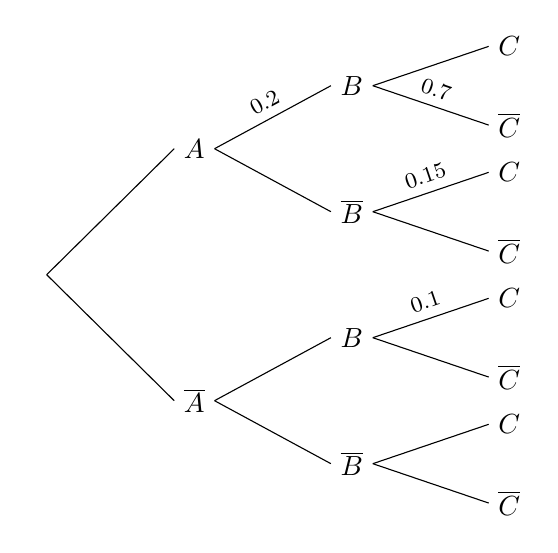
\begin{tikzpicture}[
grow=right,
sloped,
level 1/.style ={level distance=2cm, sibling distance=3.2cm, parent anchor=east, child anchor=west},
level 2/.style ={level distance=2cm, sibling distance=1.6cm},
level 3/.style ={level distance=2cm, sibling distance=1cm},
prob/.style={font=\footnotesize,above}
]

\node (root) {}
child {node {$\overline A$}
child {node {$\overline B$}
child {node {$\overline C$}
}
child {node {$C$}}
}
child {node {$B$}
child {node {$\overline C$}}
child {node {$C$}  edge from parent node[prob] {$0.1$}}
}
}
child {node {$A$}
child {node {$\overline B$}
child {node {$\overline C$}}
child {node {$C$} edge from parent node[prob] {$0.15$}}
}
child {node {$B$}
child {node {$\overline C$}  edge from parent node[prob] {$0.7$}}
child {node {$C$}}
edge from parent node[prob] {$0.2$}
}
};
\end{tikzpicture}
\end{center}

Knowing that $1.5$\% of the population suffered the three diseases, that 54\% suffered none of them and that diseases $A$ and $B$ are independent:

\begin{enumerate}
\item Complete the tree labelling the branches with their probabilities.
\item Compute the probability of suffering disease $C$.
\item Compute the probability of suffering disease $B$ if it has been suffered disease $C$.
\item Compute the probability of not suffering disease $A$ it the other two have not been suffered.
\item Are the diseases $B$ and $C$ independent?
\end{enumerate}
}
%SOLUTION
{
\begin{enumerate}
\item \hfill\break

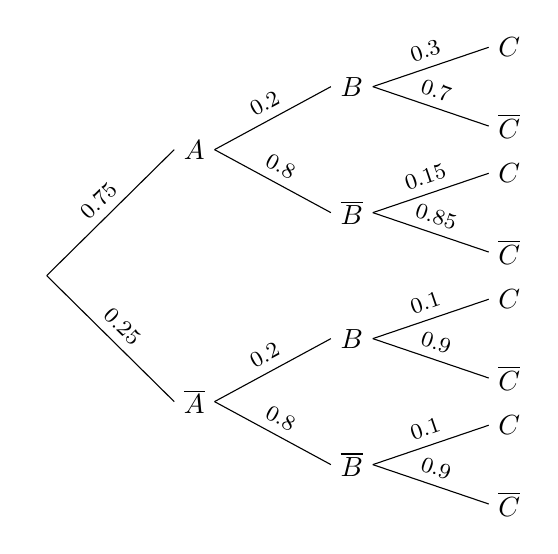
\begin{tikzpicture}[
grow=right,
sloped,
level 1/.style ={level distance=2cm, sibling distance=3.2cm, parent anchor=east, child anchor=west},
level 2/.style ={level distance=2cm, sibling distance=1.6cm},
level 3/.style ={level distance=2cm, sibling distance=1cm},
prob/.style={font=\footnotesize,above}
]

\node (root) {}
child {node {$\overline A$}
child {node {$\overline B$}
child {node {$\overline C$} edge from parent node[prob] {$0.9$}}
child {node {$C$} edge from parent node[prob] {$0.1$}}
edge from parent node[prob] {$0.8$}
}
child {node {$B$}
child {node {$\overline C$} edge from parent node[prob] {$0.9$}}
child {node {$C$}  edge from parent node[prob] {$0.1$}}
edge from parent node[prob] {$0.2$}
}
edge from parent node[prob] {$0.25$}
}
child {node {$A$}
child {node {$\overline B$}
child {node {$\overline C$} edge from parent node[prob] {$0.85$}}
child {node {$C$} edge from parent node[prob] {$0.15$}}
edge from parent node[prob] {$0.8$}
}
child {node {$B$}
child {node {$\overline C$} edge from parent node[prob] {$0.7$}}
child {node {$C$ } edge from parent node[prob] {$0.3$}}
edge from parent node[prob] {$0.2$}
}
edge from parent node[prob] {$0.75$}
};
\end{tikzpicture}

\item $P(C)=0.12$.
\item $P(B|C)=0.25$.
\item $P(\overline A | \overline B \cap \overline C)=0.7606$.
\item No, because $P(B|C)\neq P(B)$.
\end{enumerate}
}
%RESOLUTION
{
}

\newproblem{pro-56}{fis}{*}
%STATEMENT
{A study tries to determine the effectiveness of an occupational risk prevention program in jobs that require to be sit a lot of hours.
A sample of 500 individuals between 40 and 50 years that spent more than 5 hours sitting was drawn. Half of the individuals followed the prevention program (treatment group) and the other half not (control group). After 5 years it was observed that 12 individuals suffered spinal injuries in the group following the prevention program while 32 individuals suffered spinal injuries in the other group. In the following 5 years it was observed that 21 individuals suffered spinal injuries in the group following the prevention program while 48 individuals suffered spinal injuries in the other group. 

\begin{enumerate}
\item Compute the cumulative incidence of spinal injuries in the total sample after 5 years and after 10 years.
\item Compute the absolute risk of suffering spinal injuries in 10 years in the treatment and control groups.
\item Compute the relative risk of suffering spinal injuries in 10 years in the treatment group compared to the control group. Interpret it.
\item Compute the odds ratio of suffering spinal injuries in 10 years in the treatment group compared to the control group. Interpret it.
\item Which statistics, the relative risk or the odds ratio, is more suitable in this study? Justify the answer.
\end{enumerate}
}
%SOLUTION
{
\begin{enumerate}
\item Cumulative incidence after 5 years: $R(D)=0.088$. Cumulative incidence after 10 years: $R(D)=0.226$.
\item Risk in the treatment group: $R_T(D)=0.132$. Risk in the control group: $R_C(D)=0.32$.
\item $RR(D)=0.4125$. Thus, the risk of suffering spinal injuries is less than half following the prevention program. 
\item $OR(D)=0.3232$. Thus, the odd of suffering spinal injuries is less than one third following the prevention program.
\item Since the study is prospective and we can estimate the prevalence of $D$, both statistics are suitable, but relative risk is easier to interpret.
\end{enumerate}
}
%RESOLUTION
{
}